\section{Branch attack}
\label{sect:branch}
In this section we will explain an attack that can be done by a malicious node M.
The attack consists of obscuring a part of his transaction history.
M creates a new branch of his transaction history that is more favourable to him.

\subsection{Alternating partial transaction history}
A malicious node M has his own chain of transactions
and he wants to falsify his transactions after a certain point.
He wants to rewrite his transaction history from that point and create an alternate transaction history.
M wants to do this to whitewash his reputation.
The node can simply choose to forget and obscure blocks after that point.
A new branch will be created by chaining new blocks to the desired point in history.

\begin{figure}
	\centerline{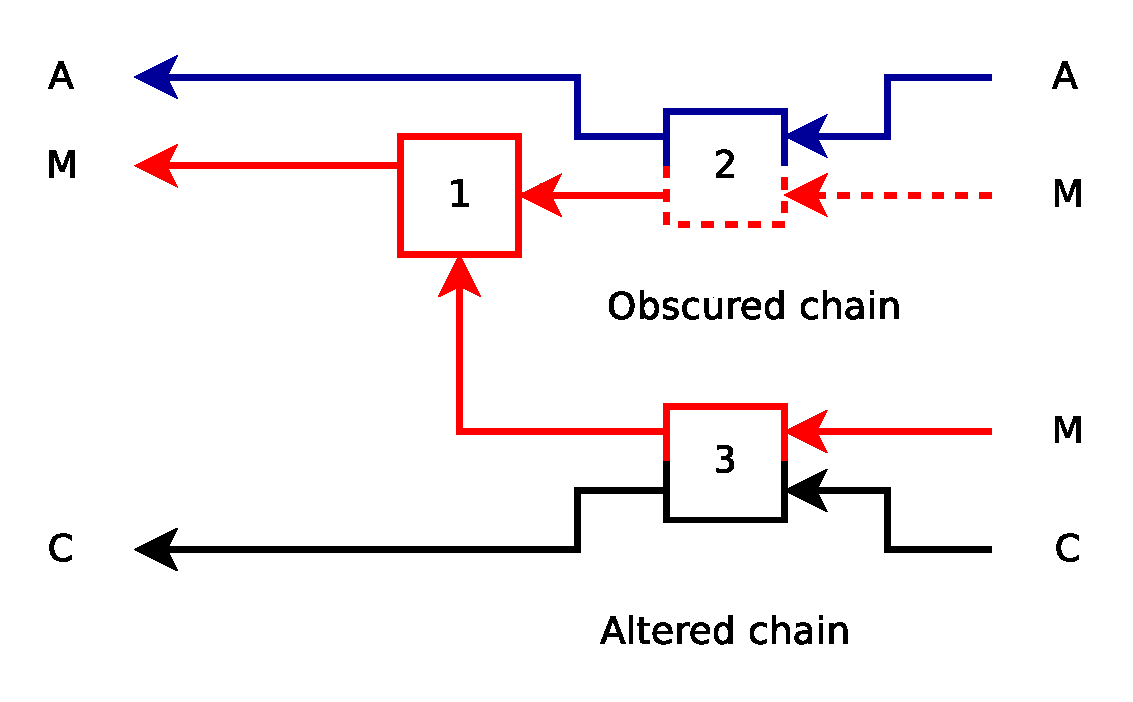
\includegraphics[scale=0.3]{problems/figs/branch.eps}}
	\caption{Example of a branch created by M.}
	\label{fig:problem-branch-obscure}
\end{figure}

In Figure \ref{fig:problem-branch-obscure} an example can be seen of a branch created by M.
In this example M tries to obscure block 2 and any subsequent blocks from C.
When C requests the transaction history of M, M will only send the transaction history up to block 1.
When M and C create a block together,
M will reuse the hash of block 1 in the new block.
For clarity of the diagram, the node interacting with M in block 1 is not displayed.

Now malicious node M does have the problem that not only he knows his transaction history.
When M interacted with node A a block was created that M tries to obscure.
A has this block in his own chain
and therefore knows about it being part of the transaction history of M.
This can be seen in the example in Figure \ref{fig:problem-branch-obscure}.

M will want to reduce the likelyhood of the detection of his fraud.
If his fraud is detected, he might be punished and no longer to continue his abuse.
The first way to minimize detection is to choose
to only interact with new nodes that do not know about the alternate part of the transaction history.
Nodes that have requested an alternate part of the transaction history
or that have been interacted directly with are no longer interacted with.
In a sufficiently healthy network this will result in node M being able to find new nodes to help him.

\begin{figure}
	\centerline{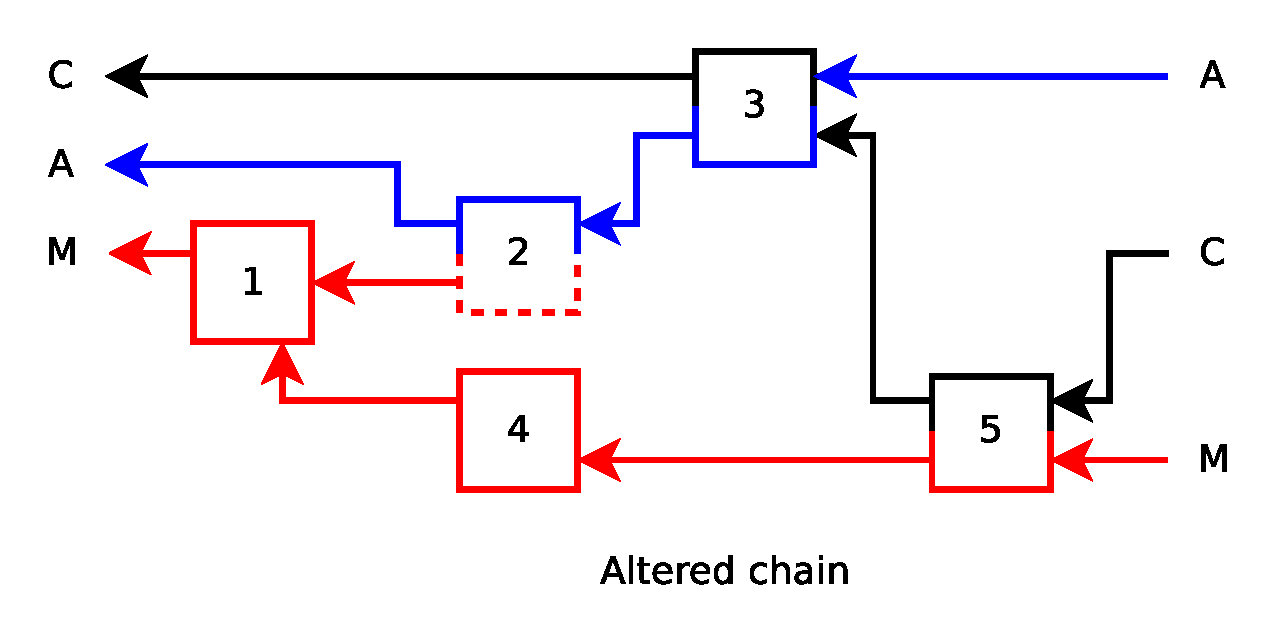
\includegraphics[scale=0.3]{problems/figs/branch-fraud-detected.eps}}
	\caption{Detectable fraud by C.}
	\label{fig:problem-branch-preknowledge}
\end{figure}

There is another example that will expose the fraud of M.
This example can be seen in Figure \ref{fig:problem-branch-preknowledge}.
A node C might still exposes the cheating of M by chance.
C can have an interaction with node A by coincidence.
Before creating block 3 C will request the transaction history of node A containing an obscured block of M.
Now when M wants to interact with C, M will want to create block 5.
When C requests the full transaction history of M, it will detect that the transaction history of M no longer contains block 2.
This exposes the fraud of M.

But C will have no sure way of exposing this type of fraud by his own doing,
except for requesting every transaction history of every node in the system.
This is in a way a common, full transaction history and was chosen to be avoided by the design to become more scalable.
C can limited the possibility of the attack by increasing his knowledge by collecting more transaction history of other nodes.
If node A or B stop participating and exit the network,
then C will have no way of detecting the fraud by M.

The second way M can limit the exposure of his cheating is in a more sophisticated way.
He can present several, different transaction history to different nodes.
M will continue keeping track of the unmodified transaction history.
When M wants to interact with A or B, both knowing this transaction history, he will present this transaction history.
So M can still interact with A and B.
But when interacting with C he will present his alternate transaction history.
C will only expose the fraud in the same way as previously.

This attack can always be done M and is not limited to circumstances.
Also the attack is not limited and M can try to fool any number of other nodes C.
As shown in Figure \ref{fig:branch-multiple}.

\begin{figure}
	\centerline{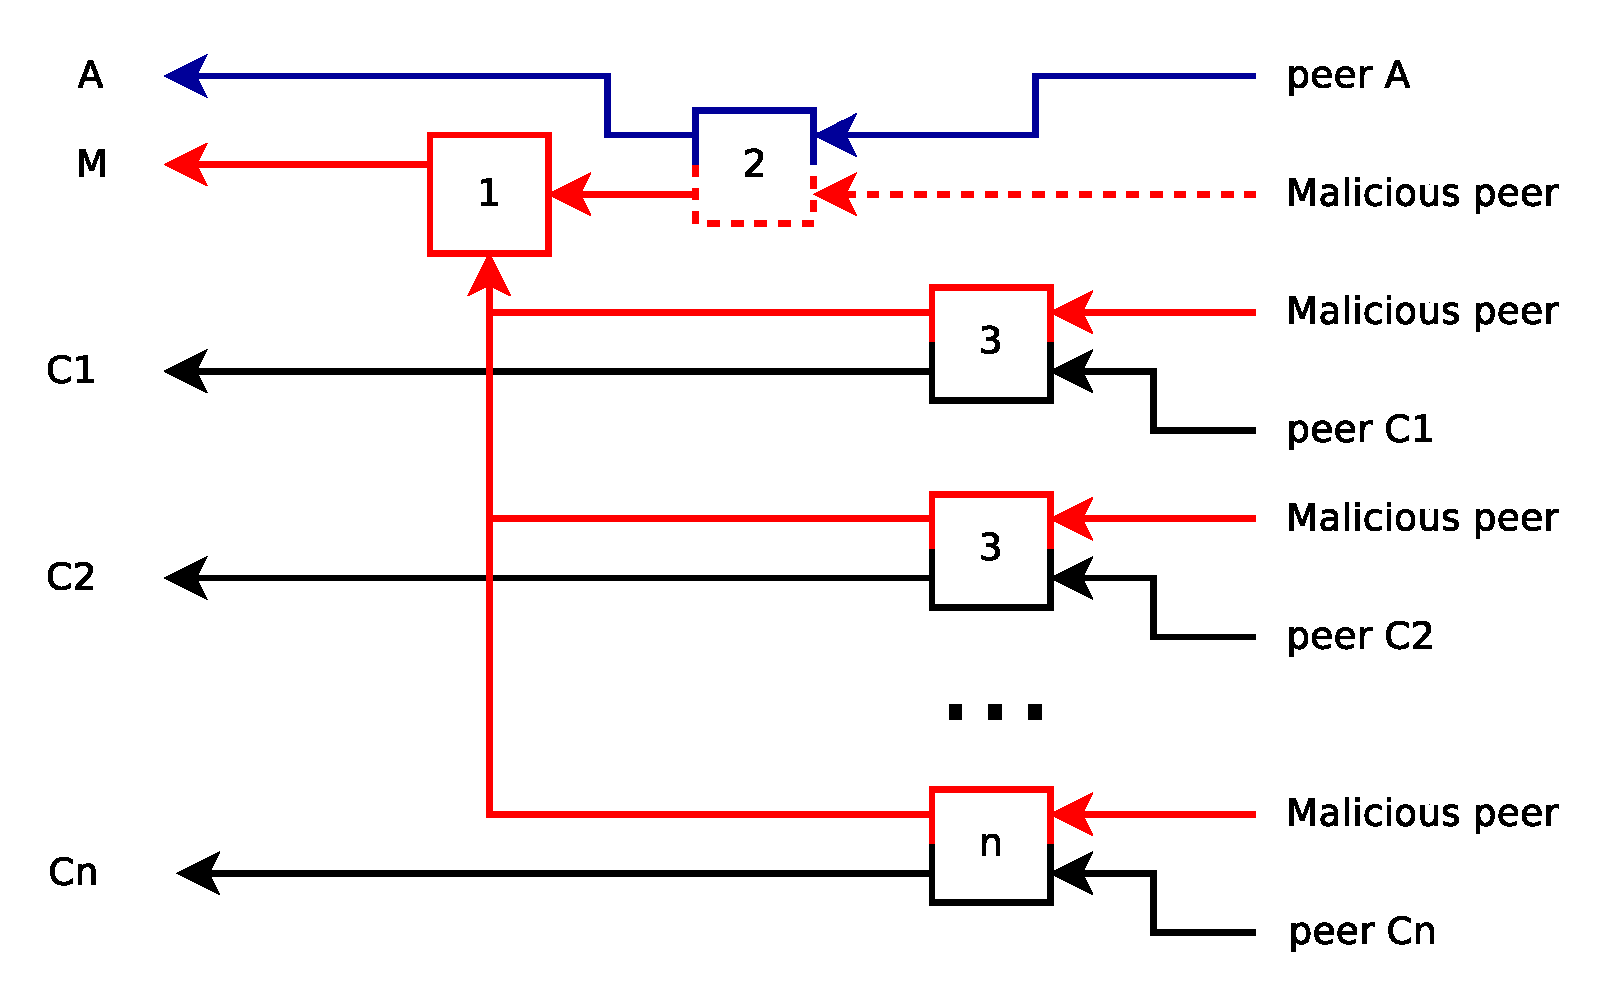
\includegraphics[scale=0.3]{problems/figs/branch-multiple.eps}}
	\caption{Example of multiple branches created by M.}
	\label{fig:branch-multiple}
\end{figure}

The likelyhood of exposing this attack depends on several factors
and will be the only factor to limit M in performing this fraud.
The likelihood depends on:
\begin{itemize}
\item Size of the network
\item Likelihood of interactions between A or B and C
\end{itemize}

These properties will influence the chance of C coming across an obscured block.

\subsection{Punishment of this attack}
When the fraud is detected by C, then currently only C can punish M by no longer interacting with him.
There is currently no way of making it globally known to every node in the network that fraud was committed.
So only M is punished by C and can continue his abuse of other nodes in the network.

A proposal for the future, that is already currently worked on, is to construct an additional network
where the discovery of the fraud can be announced.
Proof of the fraud is easily to distribute and cannot be repudiated by the malicious node.
The proof of the fraud is two blocks containing the same previous hash.
The proof cannot be repudiated, because it contains two signatures by the malicious node.
See section \ref{sect:repudiation} for more explanation.
To increase the likelyhood of detection every node will walk the network to look for fraud.